%----------------------------------------------------------------------------------------
%	PACKAGES AND OTHER DOCUMENT CONFIGURATIONS
%----------------------------------------------------------------------------------------

\documentclass[11pt]{scrartcl} % Font size

%%%%%%%%%%%%%%%%%%%%%%%%%%%%%%%%%%%%%%%%%
% Wenneker Assignment
% Structure Specification File
% Version 2.0 (12/1/2019)
%
% This template originates from:
% http://www.LaTeXTemplates.com
%
% Authors:
% Vel (vel@LaTeXTemplates.com)
% Frits Wenneker
%
% License:
% CC BY-NC-SA 3.0 (http://creativecommons.org/licenses/by-nc-sa/3.0/)
% 
%%%%%%%%%%%%%%%%%%%%%%%%%%%%%%%%%%%%%%%%%

%----------------------------------------------------------------------------------------
%	PACKAGES AND OTHER DOCUMENT CONFIGURATIONS
%----------------------------------------------------------------------------------------

\usepackage{amsmath, amsfonts, amsthm} % Math packages

\usepackage{listings} % Code listings, with syntax highlighting

\usepackage{graphicx} % Required for inserting images

\usepackage{booktabs} % Required for better horizontal rules in tables

\usepackage{dirtytalk} % Required for quoting.

\usepackage{float} % Added for hard placement of images.

\usepackage[dvipsnames]{xcolor} % Added for extra colors.

\usepackage{tikz} % For colored boxes and more.

\numberwithin{equation}{section} % Number equations within sections (i.e. 1.1, 1.2, 2.1, 2.2 instead of 1, 2, 3, 4)
\numberwithin{figure}{section} % Number figures within sections (i.e. 1.1, 1.2, 2.1, 2.2 instead of 1, 2, 3, 4)
\numberwithin{table}{section} % Number tables within sections (i.e. 1.1, 1.2, 2.1, 2.2 instead of 1, 2, 3, 4)

\usepackage{enumitem} % Required for list customisation
\setlist{noitemsep} % No spacing between list items

\usepackage[main=greek, english]{babel}

%----------------------------------------------------------------------------------------
%	DOCUMENT MARGINS
%----------------------------------------------------------------------------------------

\usepackage{geometry} % Required for adjusting page dimensions and margins

\geometry{
	paper=a4paper, % Paper size, change to letterpaper for US letter size
	top=2.5cm, % Top margin
	bottom=3cm, % Bottom margin
	left=3cm, % Left margin
	right=3cm, % Right margin
	headheight=0.75cm, % Header height
	footskip=1.5cm, % Space from the bottom margin to the baseline of the footer
	headsep=0.75cm, % Space from the top margin to the baseline of the header
	%showframe, % Uncomment to show how the type block is set on the page
}

%----------------------------------------------------------------------------------------
%	FONTS
%----------------------------------------------------------------------------------------

\usepackage[utf8]{inputenc} % Required for inputting international characters
\usepackage[T1]{fontenc} % Output font encoding for international characters

\usepackage{XCharter} % Use the XCharter fonts


%----------------------------------------------------------------------------------------
%	SECTION TITLES
%----------------------------------------------------------------------------------------

\usepackage{sectsty} % Allows customising section commands

\sectionfont{\vspace{6pt}\centering\normalfont\scshape} % \section{} styling
\subsectionfont{\normalfont\bfseries} % \subsection{} styling
\subsubsectionfont{\normalfont\itshape} % \subsubsection{} styling
\paragraphfont{\normalfont\scshape} % \paragraph{} styling

%----------------------------------------------------------------------------------------
%	HEADERS AND FOOTERS
%----------------------------------------------------------------------------------------

\usepackage{scrlayer-scrpage} % Required for customising headers and footers

\ohead*{} % Right header
\ihead*{} % Left header
\chead*{} % Centre header

\ofoot*{} % Right footer
\ifoot*{} % Left footer
\cfoot*{\pagemark} % Centre footer

\newcommand{\img}[1] % maybe add a caption to this
{
    \begin{center}
        \fcolorbox{black}{white}{\includegraphics[width=\textwidth]{#1}}
    \end{center}

}

% Helper Macros

\newcommand{\en}[1]{\foreignlanguage{english}{#1}}
\newcommand{\src}[1]{{\texttt{#1}}}


% Extra Formatting

\setlength{\parindent}{0em}
\setlength{\parskip}{0em}


% Code Listing Style

\lstdefinestyle{code}{
  belowcaptionskip=1\baselineskip,
  breaklines=true,
  frame=LRTB,
  xleftmargin=\parindent,
  showstringspaces=false,
  basicstyle=\ttfamily,
  keywordstyle=\bfseries\color{green!40!black},
  commentstyle=\itshape\color{purple!40!black},
  identifierstyle=\color{black},
  stringstyle=\color{orange},
}


\newcommand{\lstcode}[3]
{
    \begin{otherlanguage}{english}
    \lstinputlisting[language=#2, frame=single, style=code, caption=#3]{#1}
    \end{otherlanguage}
}
 % Include the file specifying the document structure and custom commands
\usepackage{multirow}
\usepackage{array}
\usepackage{subcaption}
\usepackage{textcomp}
\usepackage{algorithm}
\usepackage{algpseudocode}

\usetikzlibrary{positioning}

\usepackage{titling}

\setcounter{footnote}{0}
\renewcommand{\thefootnote}{\arabic{footnote}}

% Define a macro to create a table with fixed column widths
\newcolumntype{C}[1]{>{\centering\arraybackslash}p{#1}}

\usepackage{hyperref}
\hypersetup{
    colorlinks=true,
    linkcolor=blue,
    filecolor=magenta,      
    urlcolor=cyan,
}

\definecolor{diffstart}{named}{Apricot}
\definecolor{diffincl}{named}{Green}
\definecolor{diffrem}{named}{Red}

\usepackage{listings}
  \lstdefinelanguage{diff}{
    basicstyle=\ttfamily\small,
    morecomment=[f][\color{diffstart}]{@@},
    morecomment=[f][\color{diffincl}]{+\ },
    morecomment=[f][\color{diffrem}]{-\ },
  }

\definecolor{codegreen}{rgb}{0,0.6,0}
\definecolor{codegray}{rgb}{0.5,0.5,0.5}
\definecolor{codepurple}{rgb}{0.58,0,0.82}
\definecolor{backcolour}{rgb}{0.95,0.95,0.92}
\definecolor{codeblue}{rgb}{0,0,0.8}

\lstdefinestyle{mystyle}{
    backgroundcolor=\color{backcolour},   
    commentstyle=\color{codegreen},
    keywordstyle=\color{codeblue},
    numberstyle=\tiny\color{codegray},
    stringstyle=\color{codepurple},
    basicstyle=\ttfamily\footnotesize,
    breakatwhitespace=false,         
    breaklines=true,                 
    captionpos=b,                    
    keepspaces=true,                 
    numbers=left,                    
    numbersep=5pt,                  
    showspaces=false,                
    showstringspaces=false,
    showtabs=false,                  
    tabsize=2
}
\usepackage{tocloft}
\renewcommand{\cftsecfont}{\normalfont}
\renewcommand{\cftsecpagefont}{\normalfont}
\addto\captionsgreek{\renewcommand{\contentsname}{\normalfont Περιεχόμενα}}

\lstset{style=mystyle}

%----------------------------------------------------------------------------------------
%	TITLE SECTION
%----------------------------------------------------------------------------------------

\title{	
	\normalfont\normalsize
	\textsc{Πανεπιστήμιο Πατρών, Τμήμα Μηχανικών ΗΥ και Πληροφορικής \\Τεχνολογία λογισμικού 2023}\\ % Your university, school and/or department name(s)
	\vspace{25pt} % Whitespace
	\rule{\linewidth}{0.5pt}\\ % Thin top horizontal rule
	\vspace{20pt} % Whitespace
    {\Large Project Description v0.1}\\ % The assignment title
	\vspace{12pt} % Whitespace
	\rule{\linewidth}{0.5pt}\\ % Thick bottom horizontal rule
	\vspace{12pt} % Whitespace
    
\includegraphics[width=0.7\textwidth]{../../brand/png/logo-transparent.png}
        \rule{\linewidth}{2pt}
}
\author{
Ιωάννης Παναρίτης \thanks{Editor} \\UP1072632 \and Βασίλειος Τσούλος \thanks{Peer Review} \\UP1072605 \and Κωνσταντίνος Γιακαλλής \\UP1072533 \and \hspace{-0.9cm} Νικόλαος Χαλκιόπουλος \\ \hspace{-0.9cm}UP1072572
}



\date{} % Today's date (\today) or a custom date

%----------------------------------------------------------------------------------------
%	DOCUMENT
%----------------------------------------------------------------------------------------

\bibliographystyle{ieeetr}
\addto\captionsgreek{\renewcommand{\refname}{Αναφορές}}


\begin{document}

\maketitle
\pagebreak
\Large


\section*{Project Description}

\subsection*{Περιγραφή}

Το \src{Maintena} είναι μια φιλική προς το χρήστη εφαρμογή που στοχεύει να διευκολύνει τη συντήρηση του οχήματος για τους οδηγούς. Κάθε όχημα έχει ένα εγχειρίδιο σέρβις από τον κατασκευαστή του που αναφέρει ποιο, πόσο συχνά και πώς πρέπει να συντηρείται το όχημα. Το \src{Maintena} παρέχει μια εύχρηστη λύση που βοηθά τους οδηγούς να διατηρήσουν τη μακροζωία του οχήματός τους και την ομαλή λειτουργία του.

\subsection*{Χαρακτηριστικά}
\begin{itemize}
    \item Εισαγωγή χρήστη - Η εφαρμογή επιτρέπει στον χρήστη να εισάγει το μοντέλο αυτοκινήτου του και τα τρέχοντα χιλιόμετρα για να λάβει πληροφορίες συντήρησης ειδικά για το όχημά του.
    \item Υπενθυμίσεις συντήρησης - Η εφαρμογή θα ελέγχει συνεχώς τα χιλιόμετρα που διανύθηκαν (ή τις ώρες χρήσης για ορισμένες συσκευές) και θα παρέχει στον χρήστη τακτικές ενημερώσεις σχετικά με το πότε θα γίνει η επόμενη υπηρεσία, ποιες αλλαγές πρέπει να γίνουν, πόσο πιθανόν θα κοστίσει και πού να προμηθευτείτε ανταλλακτικά ή τη βοήθεια έμπειρου τεχνίτη.
    \item Αναβαθμίσεις απόδοσης - Το \src{Maintena} προσφέρει προτάσεις για αναβαθμίσεις για τη βελτίωση της απόδοσης του οχήματος, όπως αλλαγές φίλτρων, χαρτογράφηση εγκεφάλου και αγωνιστικά καύσιμα. Αυτές οι προτάσεις βασίζονται στις οδηγικές συνήθειες του χρήστη και στην κατάσταση του οχήματος.
    \item Ιστορικό προβλημάτων - Η εφαρμογή παρακολουθεί όλα τα ζητήματα που αντιμετώπισε το όχημα στο παρελθόν, συμπεριλαμβανομένης της ημερομηνίας του προβλήματος, του κόστους επισκευής και της τοποθεσίας του συνεργείου επισκευής.
    \item Νέος πίνακας συντήρησης - Η εφαρμογή προσαρμόζει το πρόγραμμα συντήρησης στα νέα εξαρτήματα που είναι εγκατεστημένα στο όχημα. Για παράδειγμα, ένας κινητήρας που λειτουργεί με μεγαλύτερη συμπίεση από την κανονική απαιτεί συχνότερη και καλύτερη συντήρηση.
    \item Community Discussion - \src{Maintena} παρέχει μια πλατφόρμα για τους χρήστες να συζητούν και να λύνουν σχετικές ερωτήσεις με άλλους οδηγούς και τεχνίτες.
    \item Διάγνωση οχήματος - Η εφαρμογή προσφέρει καλύτερη επίγνωση της κατάστασης και των δυνατοτήτων του οχήματος. Παρέχει μια διαγνωστική αναφορά που εντοπίζει πιθανά προβλήματα και προτείνει λύσεις για τη διατήρηση της λειτουργίας του οχήματος με τον καλύτερο δυνατό τρόπο.
\end{itemize}

\subsection*{Οφέλη}
    \begin{itemize}
        \item Άνεση - Το \src{Maintena} παρέχει έναν βολικό τρόπο παρακολούθησης του προγράμματος συντήρησης του οχήματός σας και παρέχει προτάσεις για βελτιώσεις.
        \item Οικονομία - Η εφαρμογή βοηθά στη διατήρηση της μακροζωίας του οχήματος, μειώνοντας την ανάγκη για δαπανηρές επισκευές και αντικαταστάσεις.
        \item Βελτιωμένη απόδοση - Η εφαρμογή προσφέρει προτάσεις για αναβαθμίσεις που μπορούν να βελτιώσουν την απόδοση του οχήματος, κάνοντας την οδήγηση πιο απολαυστική.
        \item Κοινότητα - Η εφαρμογή παρέχει μια πλατφόρμα στους χρήστες να συζητούν και να λύνουν σχετικές ερωτήσεις με άλλους οδηγούς και τεχνίτες.
    \end{itemize}

\pagebreak

\section*{Mock ups \cite{materialdesign}}

\begin{figure}[!htb]
\begin{subfigure}{.5\textwidth}
  \centering
  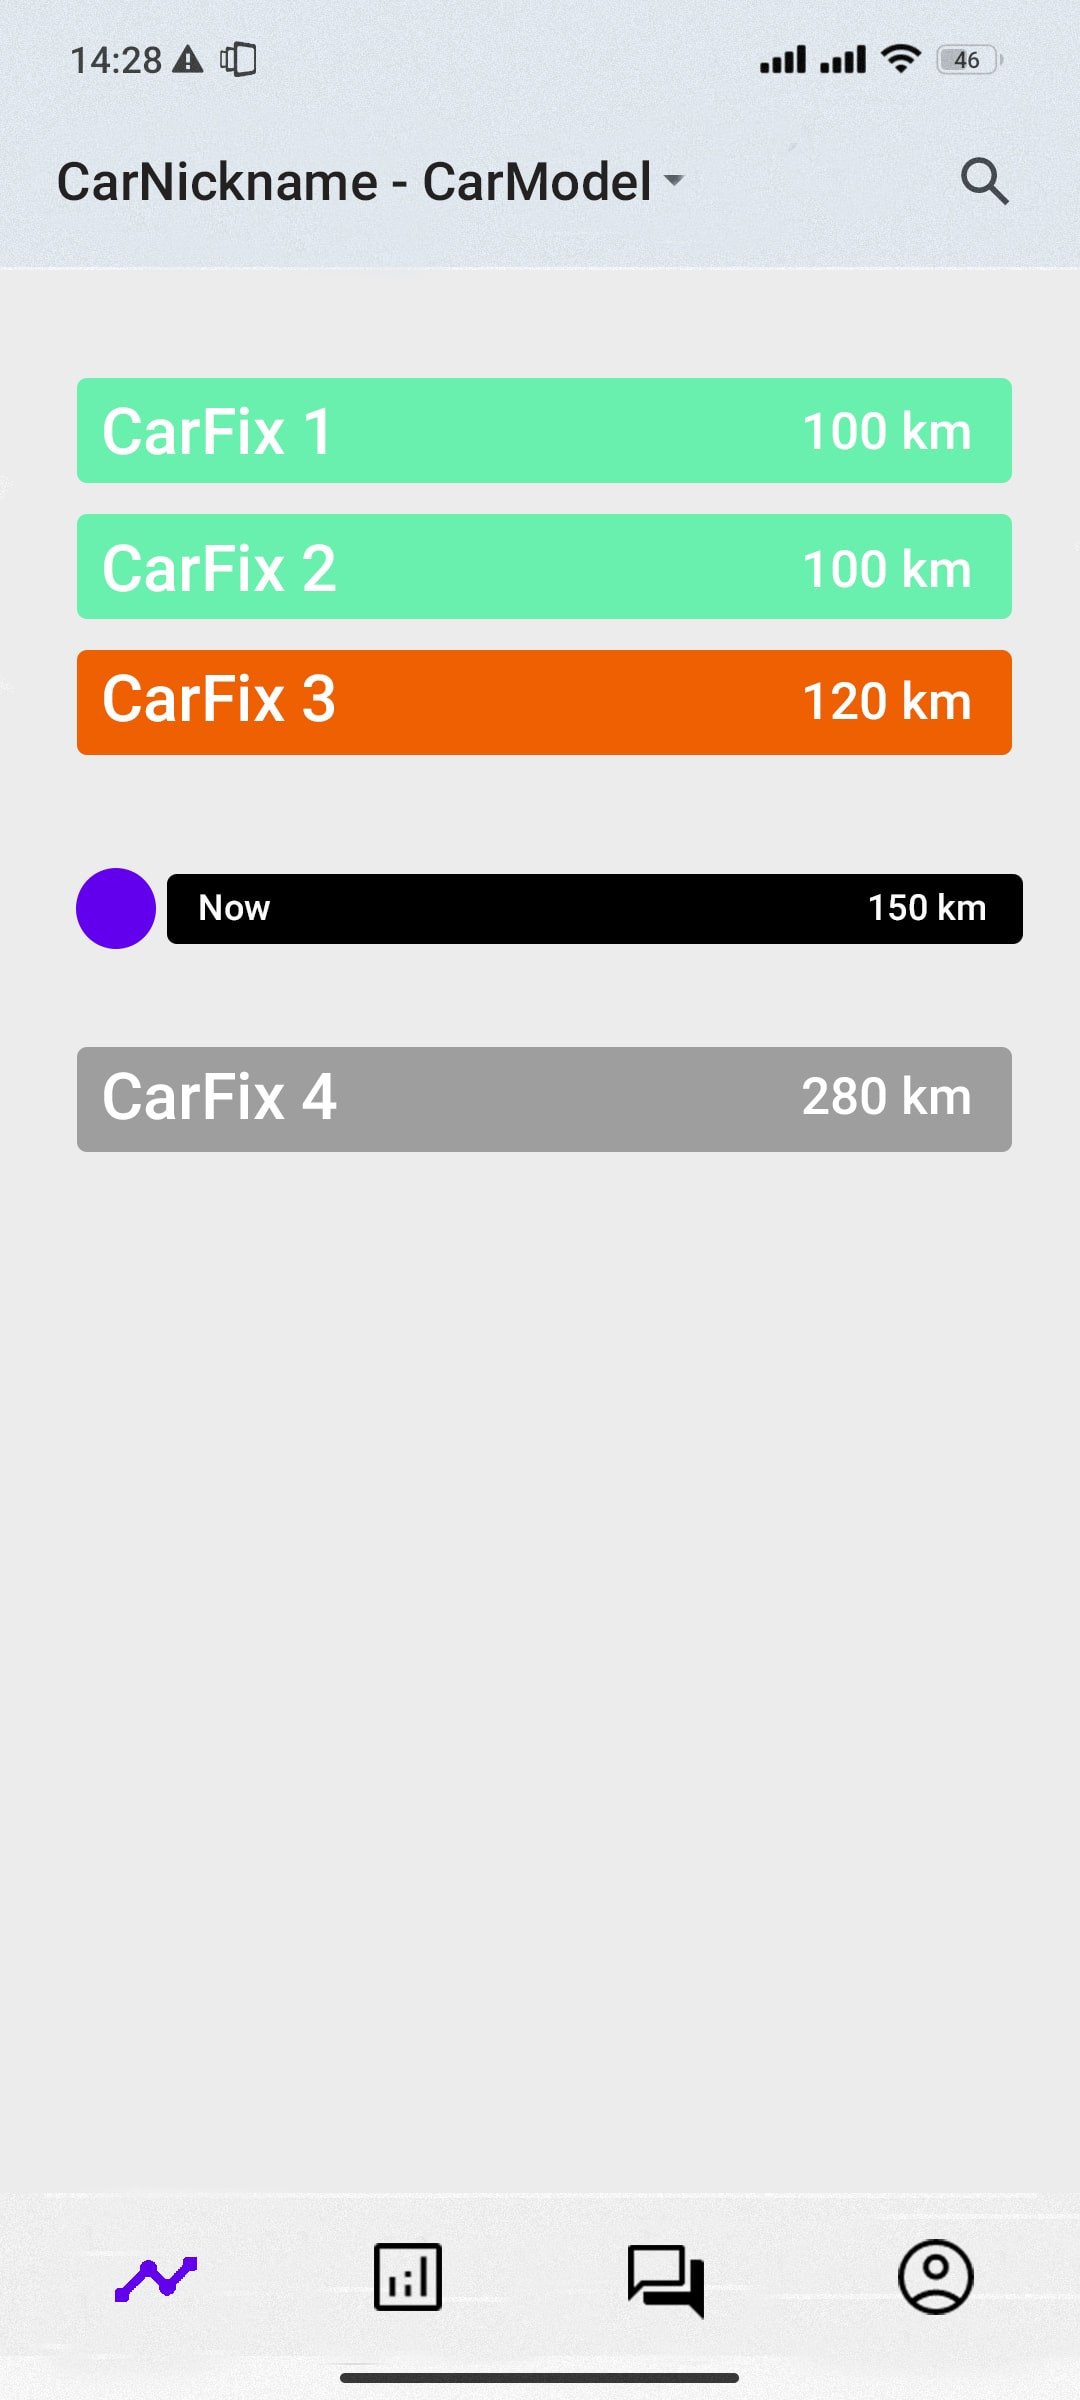
\includegraphics[width=.6\linewidth]{assets/timeline_mock_up.jpg}
  \caption{Timeline}
  \label{fig:sfig1}
\end{subfigure}%
\begin{subfigure}{.5\textwidth}
  \centering
  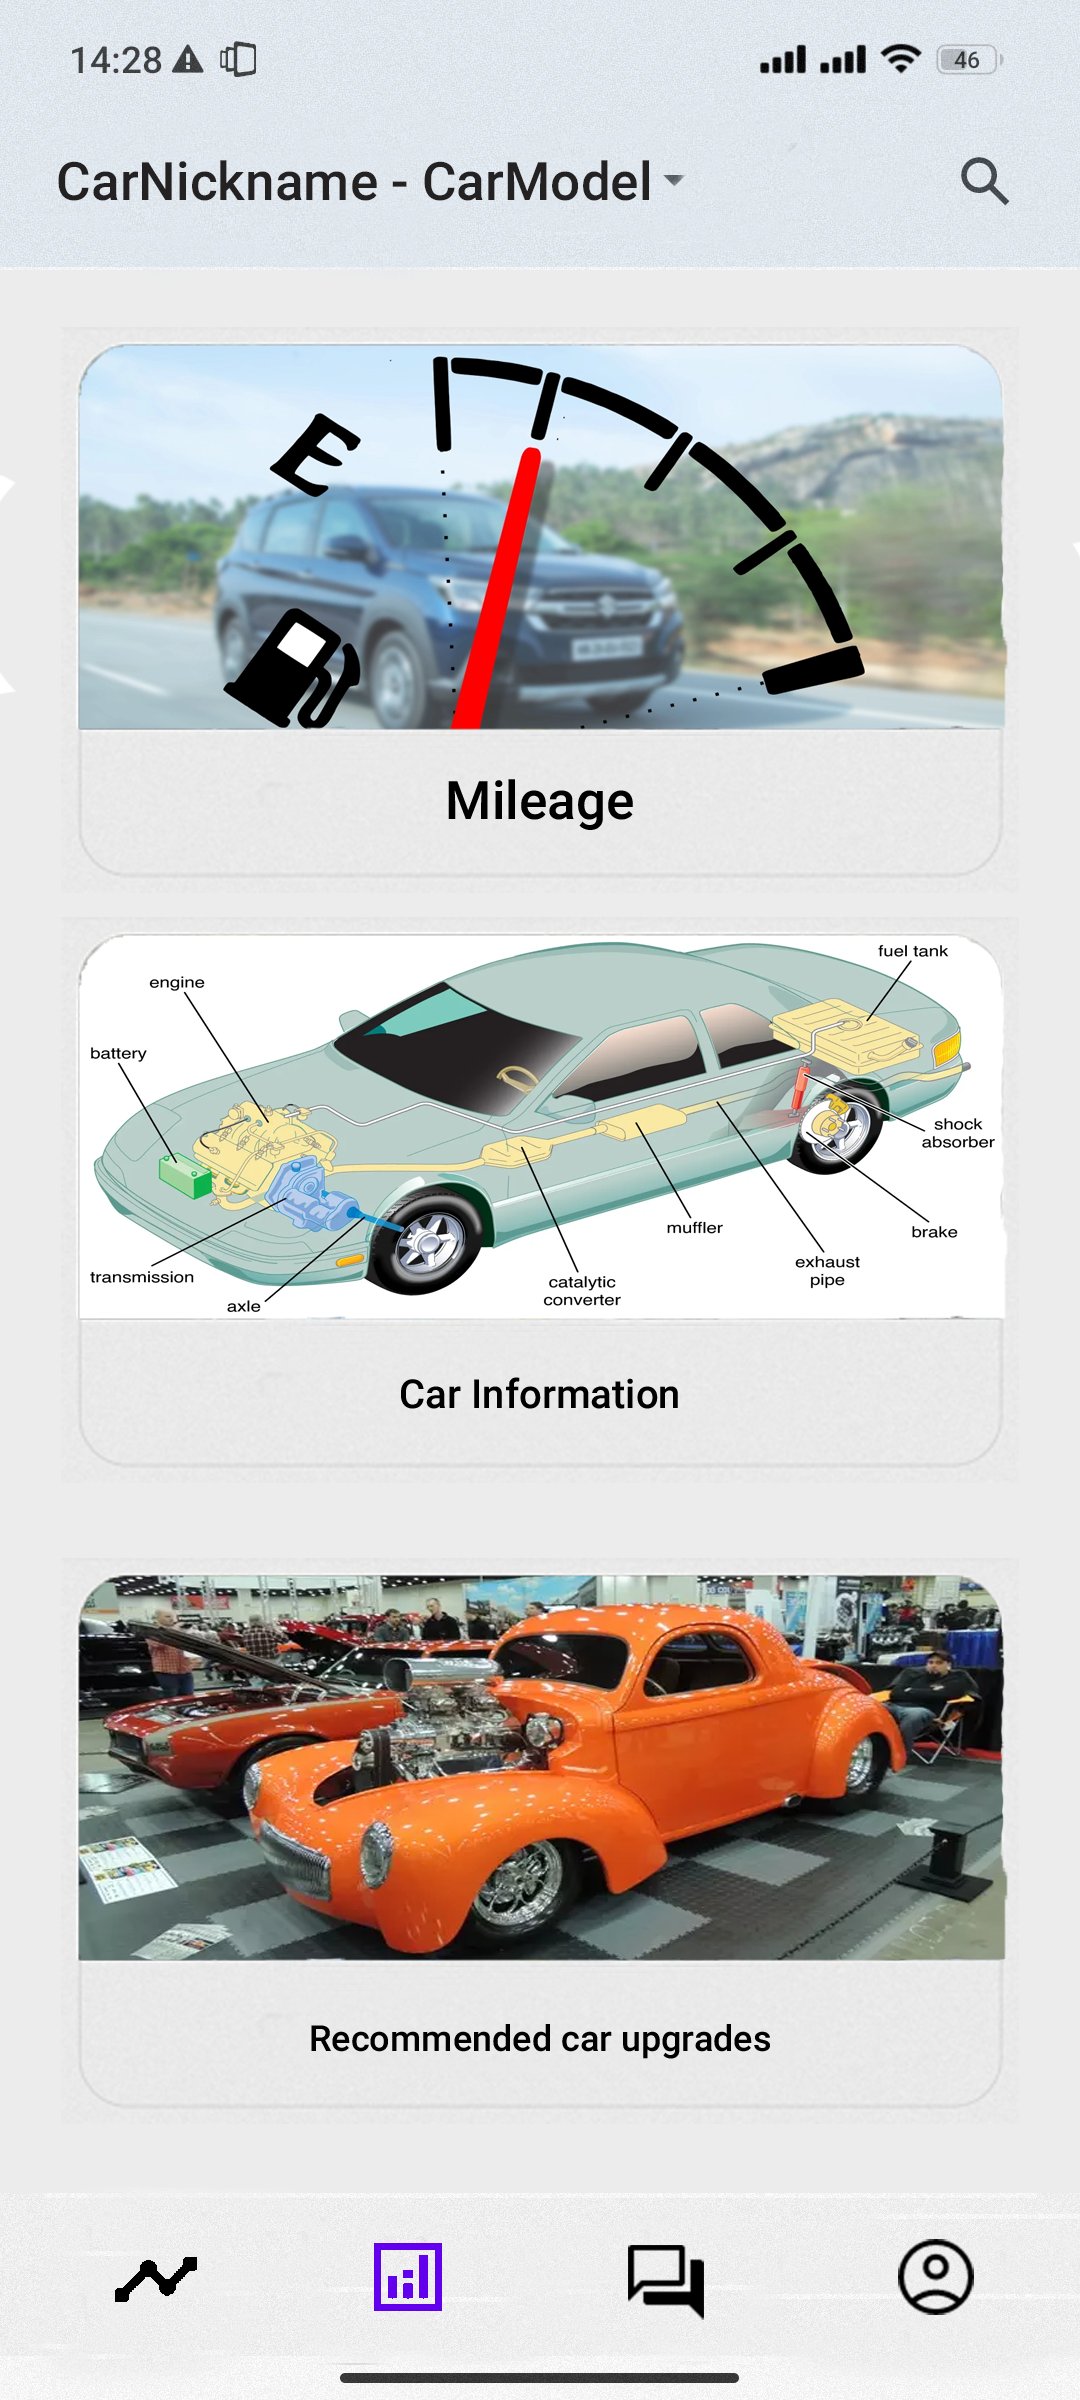
\includegraphics[width=.6\linewidth]{assets/analytics_mock_up.png}
  \caption{Analytics}
  \label{fig:sfig2}
\end{subfigure}
\label{fig:fig}
\par\bigskip % force a bit of vertical whitespace
\begin{subfigure}{.5\textwidth}
  \centering
  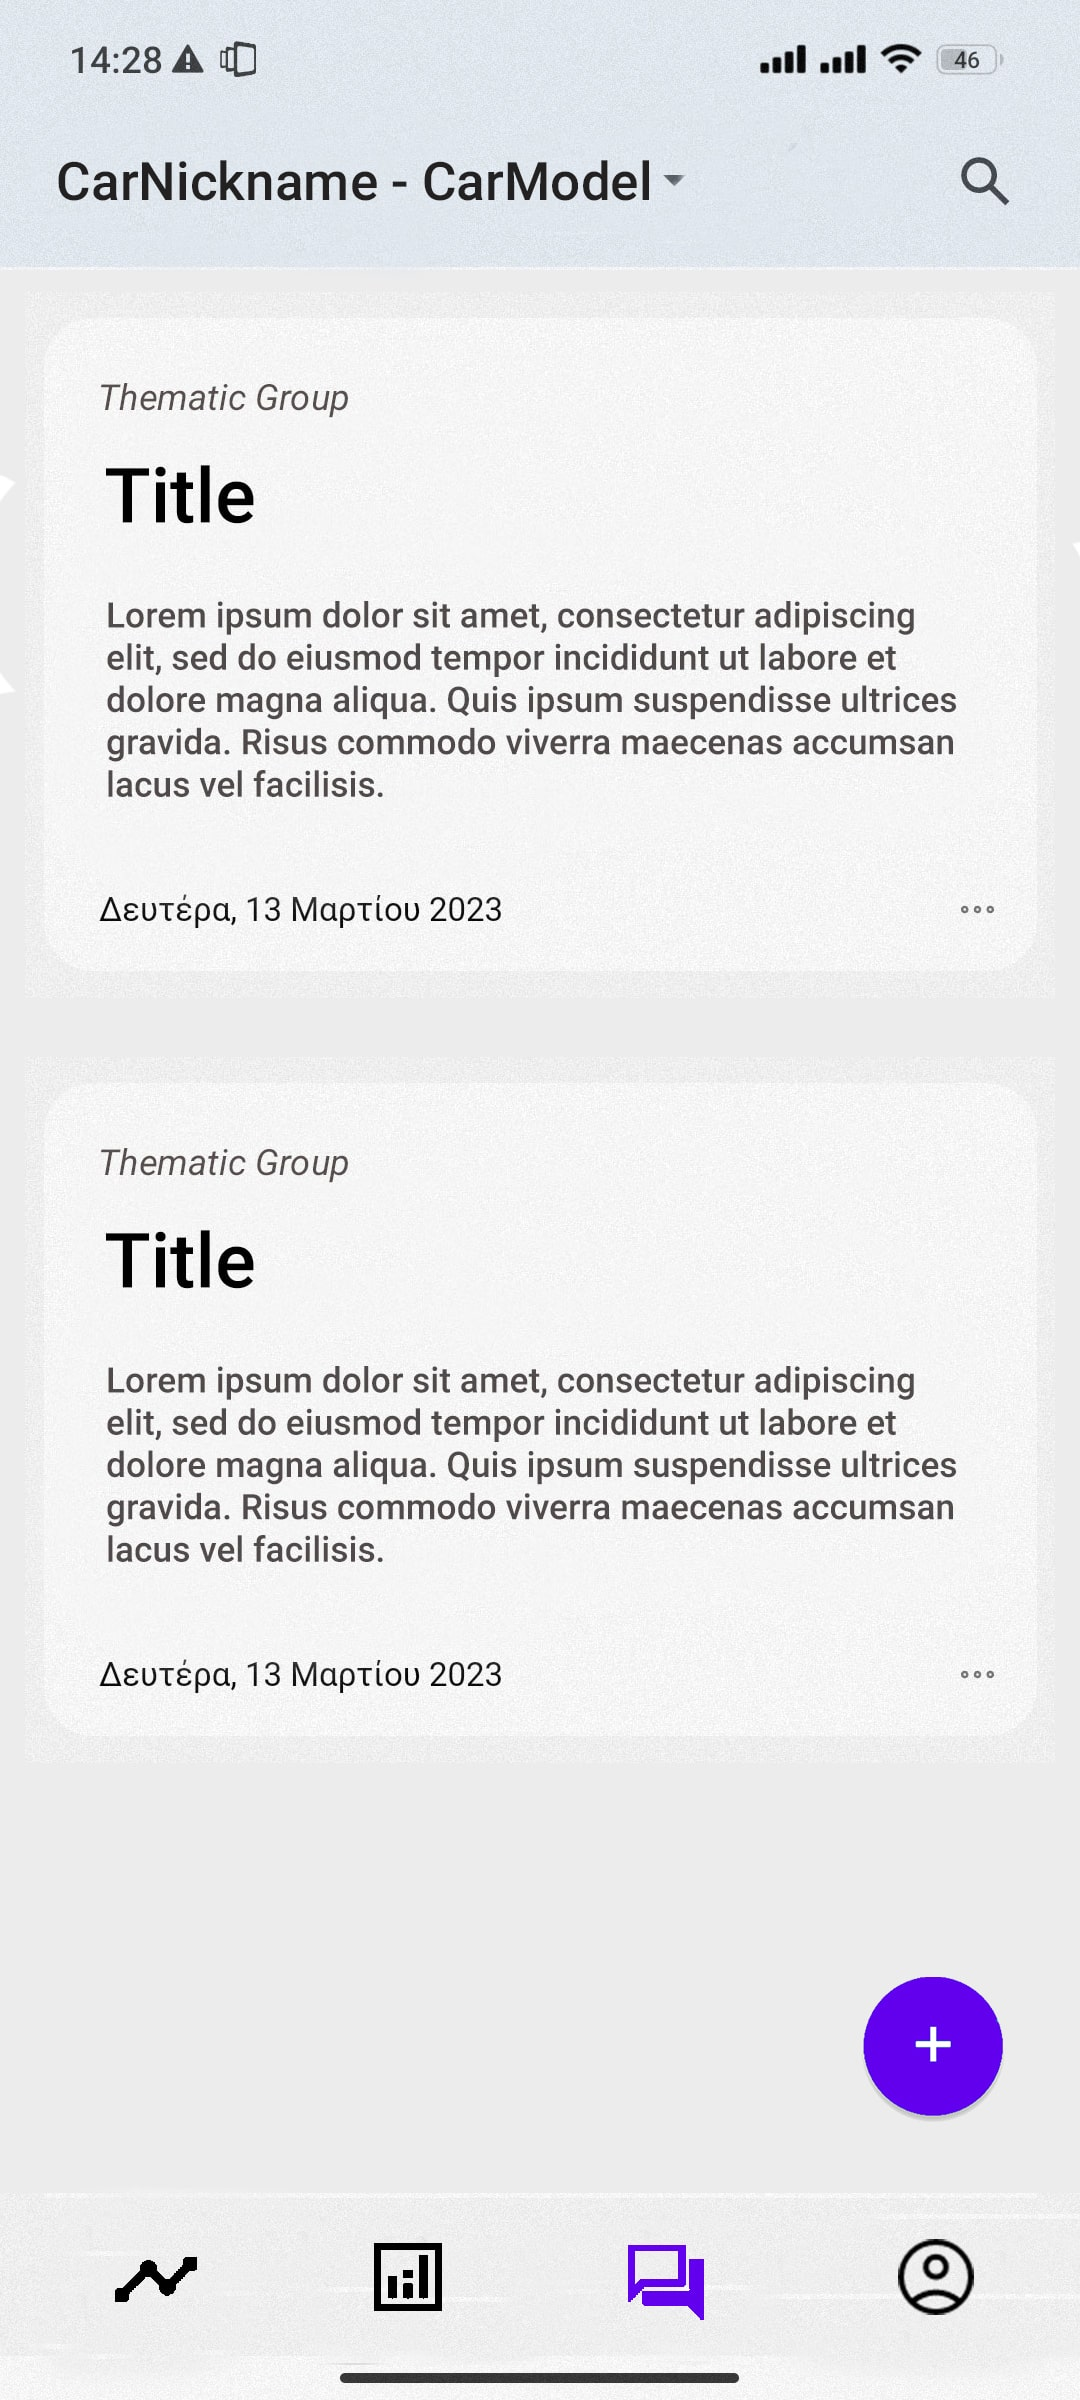
\includegraphics[width=.6\linewidth]{assets/forum_mock_up.jpg}
  \caption{Forum}
  \label{fig:sfig3}
\end{subfigure}
\label{fig:fig}
\begin{subfigure}{.5\textwidth}
  \centering
  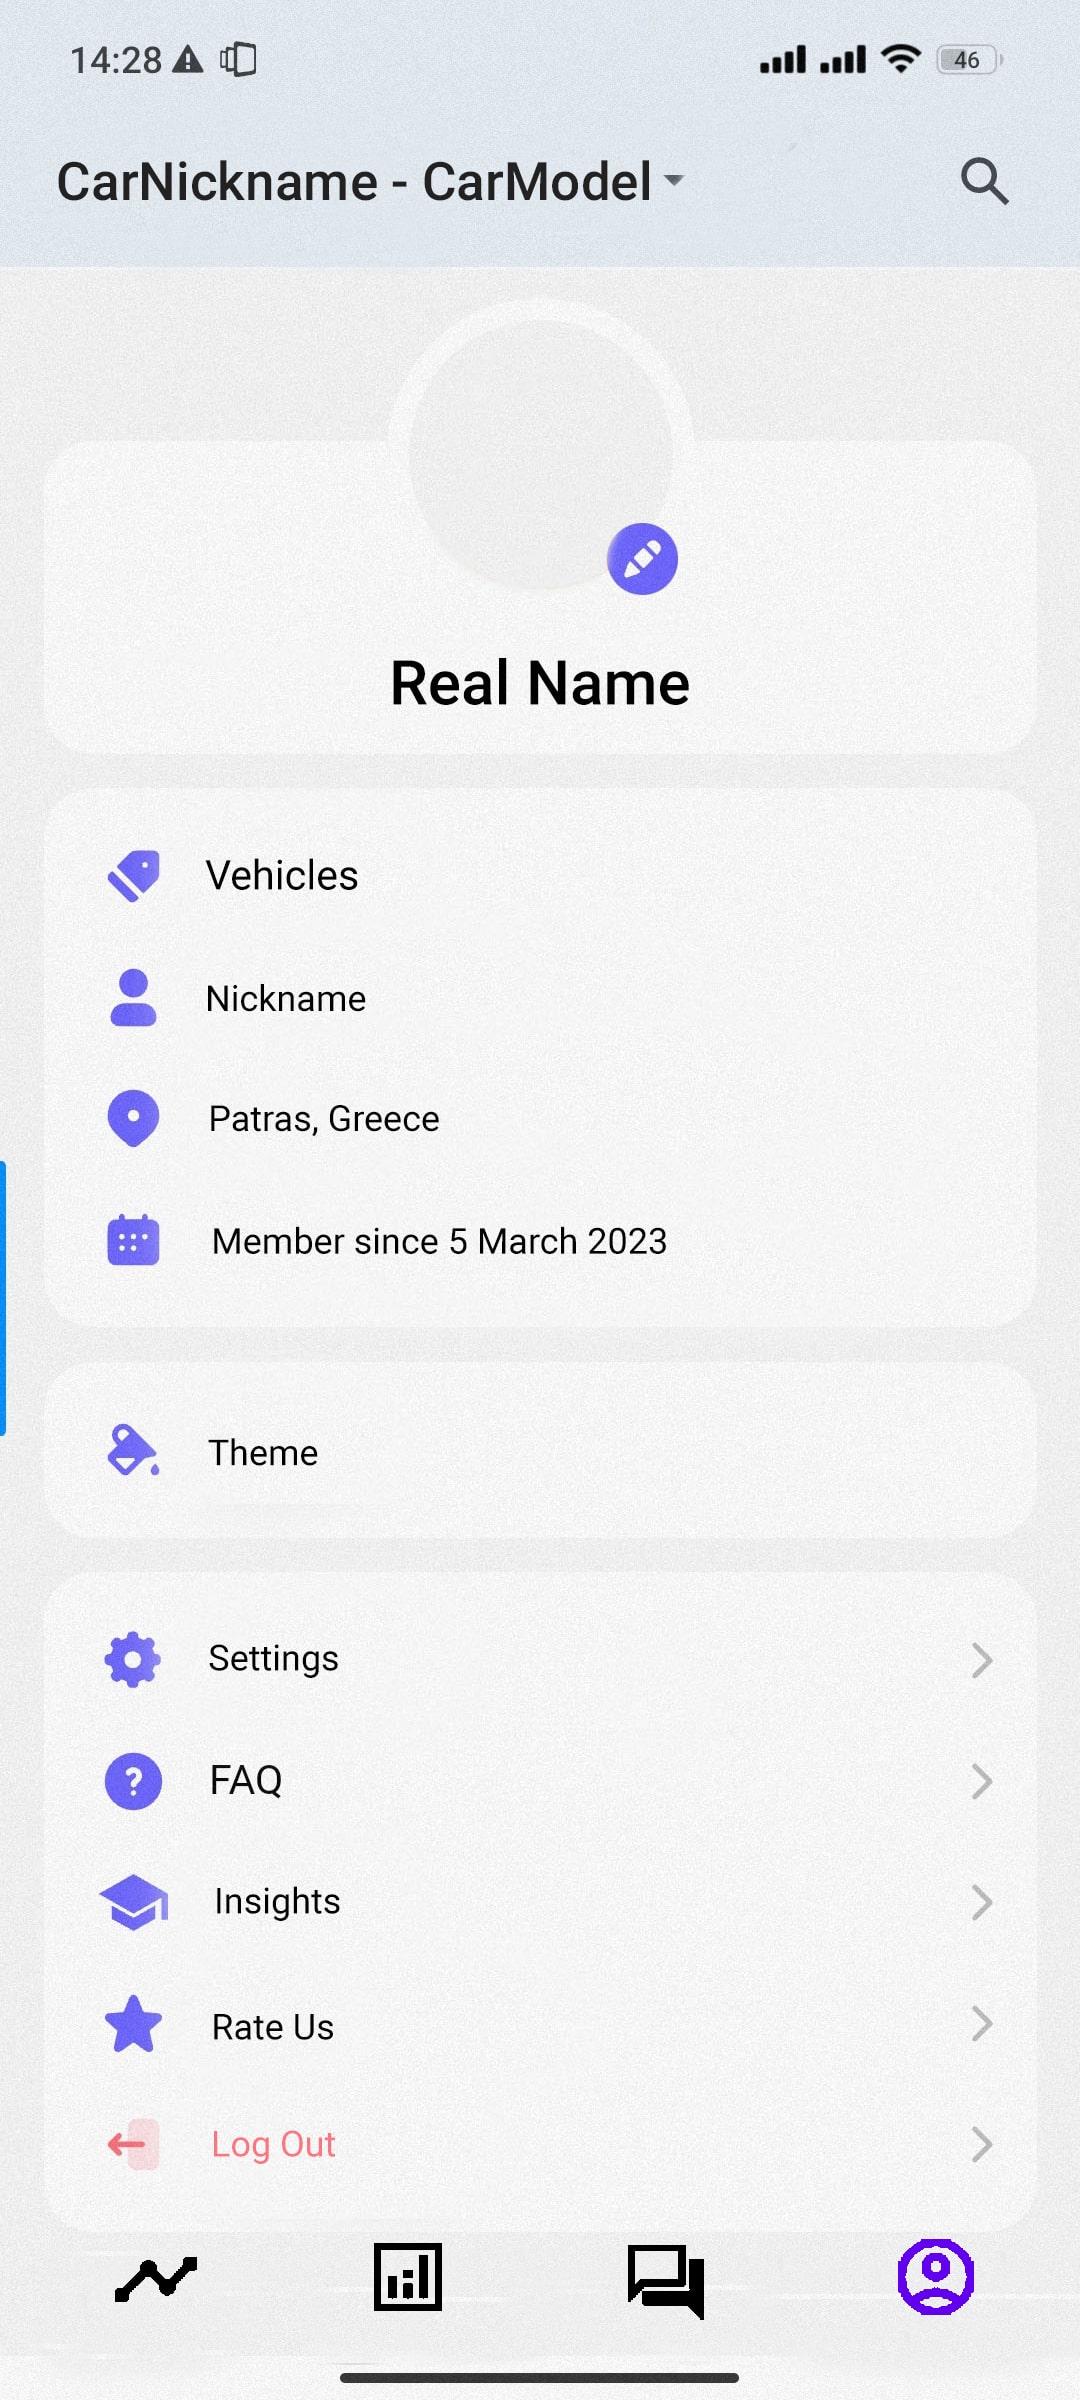
\includegraphics[width=.6\linewidth]{assets/profile_mock_up.jpg}
  \caption{Profile}
  \label{fig:sfig4}
\end{subfigure}
\label{fig:fig}
\end{figure}

\section*{Tools Used}
\begin{itemize}
    \item Συγγραφή κειμένου: Overleaf
    \item Δημιουργία Mock up: Gimp
\end{itemize}

\bibliography{bibliography}
% \cite{materialdesign}

\end{document}
